\documentclass[10pt,letterpaper]{article}
\usepackage{tools}
\usepackage{enumitem}
%\settextfont{B Nazanin}
\usepackage{lipsum}
\setlength{\parskip}{3mm}
\setlength{\parindent}{0mm}
\newcommand{\wid}{0.49\textwidth}
\newcommand{\widone}{60mm}
\begin{document}
\Large
\begin{center}
In the name of beauty

7th problem set of ComNet course
\hl
\end{center}
Q1) Determine the following statements as true or false. (Use enough reasons and explanation to support your answer)

\begin{enumerate}[label=\alph*-]
\item
The typical network-layer Internet service preserves the order of packet transmission as opposed to their eventual delivery at receiver.
\item
Both connection services in network layer and connection-oriented services in transport layer require implementations in both the end systems and routers.
\item
Routers need to only implement the layer 3 protocols.
\item
One of the major rules implemented in Routers' control plane is to manage the forwarding table.
\end{enumerate}

Q2) a. When obtaining IP address through DHCP, why do the host and the DHCP server maintain the broadcast IP address (255.255.255.255) at the steps of DHCP request and ACK?

b. Assume a NATed host with local IP address 172.17.1.39 requests for a webpage on port \#10000. What is the src. and dest. IP addresses and port numbers in the datagrams sent from the the first-hop router to the webserver and vice versa and from the router to the host and vice versa if the router maps the local IP address and port number to 10.250.96.8:80?

Q3) Consider a router that interconnects three subnets: Subnet 1, Subnet 2, and Subnet 3. Suppose all of the interfaces in each of these three subnets are required to have the prefix 223.1.17/24. Also suppose that Subnet 1 is required to support at least 60 interfaces, Subnet 2 is to support at least 90 interfaces, and Subnet 3 is to support at least 12 interfaces. Provide three network addresses (of the form a.b.c.d/x) that satisfy these constraints.

Q4) Assume the \textbf{Random Early Detection} algorithm is used for maintaining the input buffer of the input interfaces.
In brief this algorithm works as follow: The packets arrive with probability $p$ to each input interface at each timeslot. The packets have a constant length of $L$. The minimum and maximum thresholds are set to $5L$ and $8L$, respectively such that if the length of the queue falls within these thresholds, the new incoming packets are dropped with probability $1\over 5$. If the length of the queue becomes $8L$ or more, the new incoming packets are dropped with probability $1$. 

What is the probability that a newly-arrived packet is dropped?

(Hint: a queue is defined by a consecutive array of packets with no empty room between them. For further information about the Random Early Detection algorithm, you can check section 4.3.4, ``Where Does Queuing Occur?'', page 329 of ``Computer Networking; A top down approach'').

Q5) Perform the Dijkstra's algorithm for the following network to obtain the optimum path of nodes between nodes A and Z.
\begin{figure}[htbp]
\centering
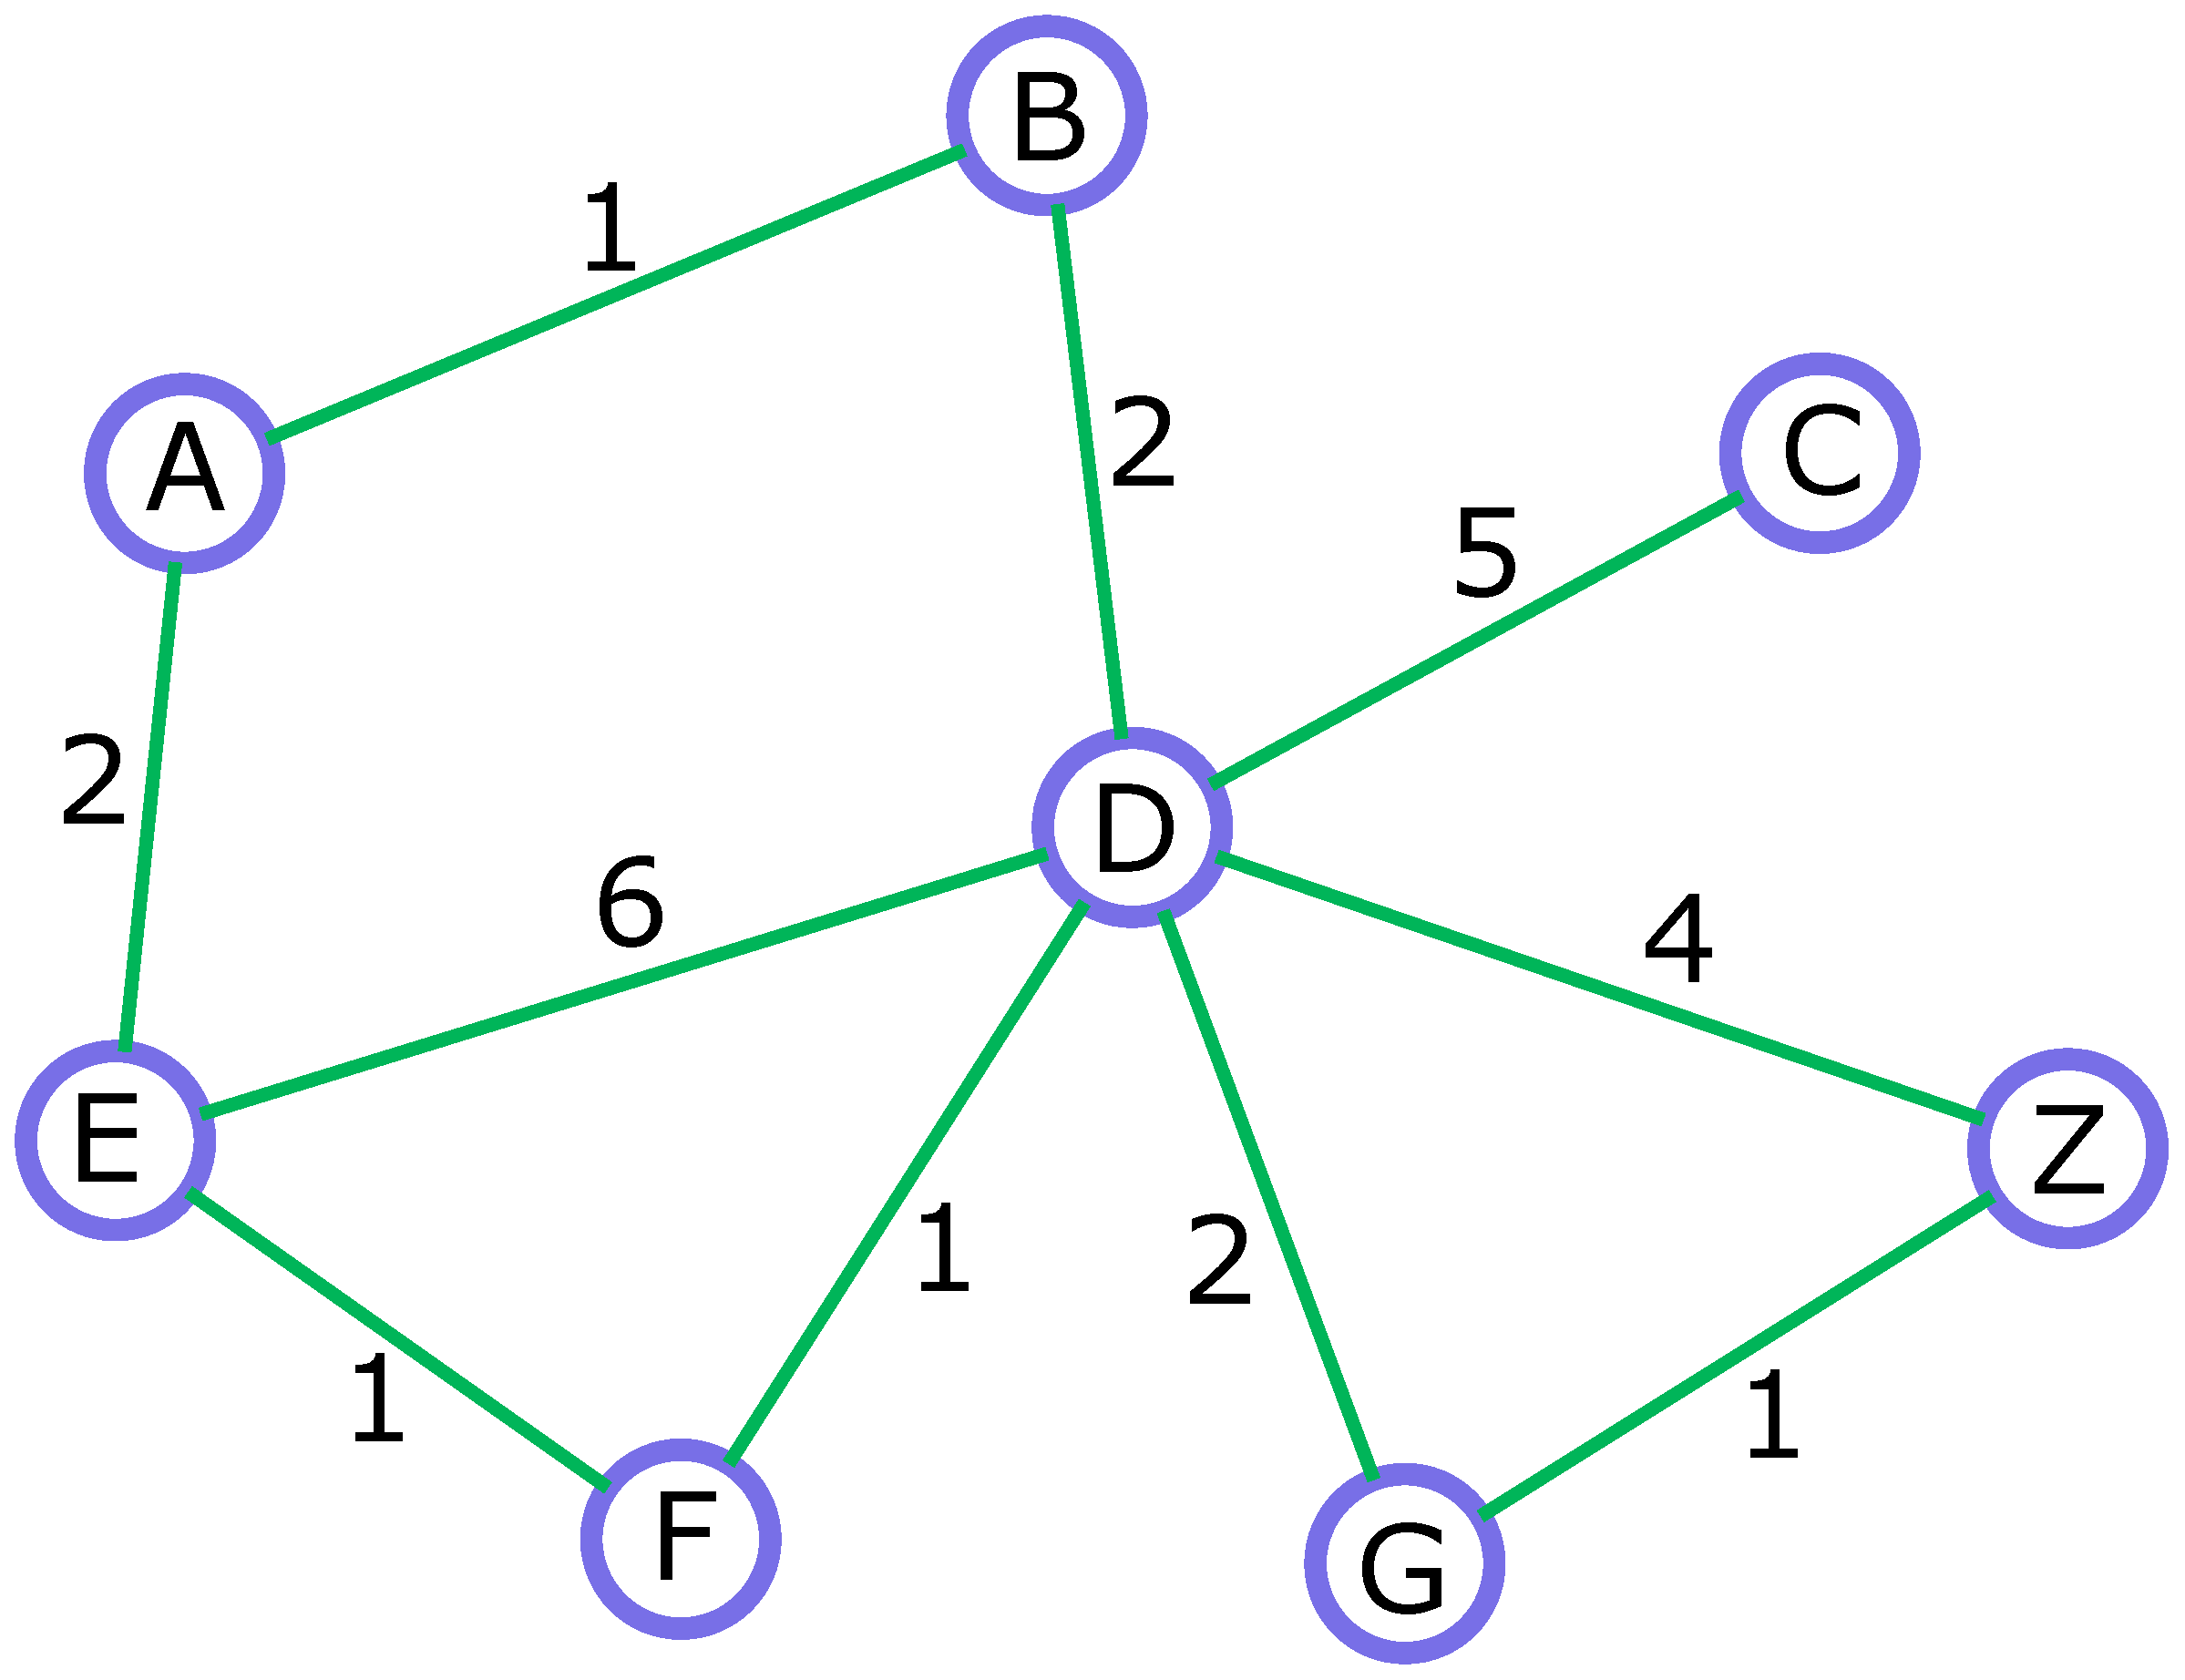
\includegraphics[width=100mm]{dij.eps}
\end{figure}
\end{document}